% =====================================================================
% Overleaf 컴파일 설정 (중요, 반드시 확인)
%   Menu > Settings > Compiler: pdfLaTeX 이 아니라 "XeLaTeX" 로 변경하세요.
%   (본문에 한글이 들어가기 때문에 kotex 패키지는 xelatex/lualatex에서만 동작합니다.
%    pdflatex로 두면 컴파일 에러가 납니다.)
%   컴파일 에러가 계속 나면 아래 \documentclass 줄을
%   \documentclass{article} 로 바꿔서 우선 내용부터 완성하세요.
% =====================================================================
\documentclass[conference]{IEEEtran}

\usepackage{kotex}           % 한글 지원 (xelatex/lualatex 필요)
\usepackage{amsmath,amssymb}
\usepackage{graphicx}
\usepackage{booktabs}
\usepackage{hyperref}
\usepackage{caption}

\title{PPO 기반 RLHF 미세조정에서 KL 계수가\\보상--다양성 트레이드오프에 미치는 영향:\\KoChatGPT 사례 연구}

\author{
  \IEEEauthorblockN{Yongseok Oh}
  \IEEEauthorblockA{ysoh1113@gmail.com}
}

\begin{document}
\maketitle

\begin{abstract}
RLHF(Reinforcement Learning from Human Feedback)의 마지막 단계인 PPO 미세조정은
보상 극대화와 원래 정책으로부터의 이탈을 억제하는 KL 페널티 사이의 트레이드오프로
정의된다. 이 트레이드오프를 통제하는 KL 계수 $\beta$는 널리 쓰이는 한국어 RLHF
튜토리얼 프로젝트인 KoChatGPT(airobotlab, 2023; ColossalAI Coati 기반)에서
검증 없이 라이브러리 기본값(0.1)으로 고정되어 있었다. 본 연구는 $\beta \in
\{0, 0.02, 0.05, 0.1, 0.3, 1.0\}$에 대한 통제된 스윕 실험과, 그중 세 조건
($\beta{=}0, 0.02, 0.1$)에 대한 2개 추가 시드 반복 실험을 수행하여, KoGPT2
기반 RLHF-PPO 미세조정에서 $\beta$가 보상, 실제 KL divergence, 생성
다양성에 미치는 영향을 정량화한다. 실험 결과 (i) 본 실험 규모(조건당
1--3개 시드, 10 episode)에서는 PPO로 미세조정한 6개 조건 모두 SFT baseline보다
평균 보상이 낮았고, (ii) 샘플 단위 반복률(repetition rate) 지표로 보면
baseline을 포함한 거의 모든 조건에서 반복 붕괴 경향이 관측되어 이 경향이
$\beta$가 아니라 SFT 단계에서부터 이어진 것으로 보이며, (iii) 시드 반복
실험에서 동일 시드 내 $\beta$ 간 차이가 시드 간 차이보다 작아, 이 규모에서는
$\beta$의 효과가 시드 분산에 의해 가려질 수 있음을 확인했다. 또한 (iv)
corpus 단위로 풀링된 distinct-n 지표가 실제로는 반복 붕괴가 있는 조건을
"다양성이 충분하다"고 잘못 판정하는 사례를 정량적으로 확인하여, 샘플 단위
반복률 지표를 보완 기준으로 제안한다.
\end{abstract}

% =====================================================================
\section{Introduction}
% =====================================================================

RLHF는 (i) supervised fine-tuning(SFT), (ii) 보상모델(RM) 학습, (iii) PPO 기반
정책 미세조정의 3단계로 구성된다. 이 마지막 단계에서 정책은 보상모델의 점수를
최대화하는 동시에, 원래 정책(SFT)으로부터 지나치게 벗어나지 않도록 KL
divergence로 정규화된다. 이 정규화의 강도를 결정하는 계수 $\beta$는 RLHF의
핵심 하이퍼파라미터임에도 불구하고, 실습/튜토리얼 목적의 오픈소스 구현체에서는
검증 없이 기본값이 그대로 쓰이는 경우가 많다.

본 연구는 ColossalAI Coati 라이브러리를 이용해 KoGPT2로 RLHF 파이프라인을
재현하는 한국어 튜토리얼 프로젝트 \textbf{KoChatGPT}~\cite{kochatgpt2023,
colossalchat2023}를 확장 대상으로 삼는다. 실제 라이브러리 소스 코드를 분석한
결과, \texttt{PPOTrainer}의 KL 계수 인자(\texttt{kl\_coef})는 기본값 0.1로
설정되어 있고, KoChatGPT 튜토리얼은 이 값을 한 번도 검증하지 않은 채 그대로
사용하고 있었다. 본 연구는 바로 이 지점 -- $\beta$가 실제로 결과에 미치는
영향 -- 을 체계적인 스윕 실험과 다중 시드 반복 실험으로 검증함으로써 기존
연구를 확장한다.

\subsection{연구 질문 및 가설}
\begin{itemize}
  \item \textbf{H1.} $\beta$가 작을수록 보상모델 점수는 높아지지만, 생성
        다양성은 낮아진다 (reward--diversity trade-off).
  \item \textbf{H2.} $\beta$가 클수록 정책이 SFT 모델에서 거의 벗어나지
        못해 보상 개선이 미미하다.
  \item \textbf{H3.} 두 극단 사이에 보상 개선 대비 텍스트 붕괴가 적은
        중간 지점이 존재한다.
\end{itemize}

\subsection{기여}
\begin{itemize}
  \item KoChatGPT의 PPO 단계에서 미검증 상태였던 KL 계수 $\beta$를
        체계적으로 스윕하고, 이를 실제 라이브러리 소스(보상 계산식, KL
        추정 방식)에 기반해 재현 가능한 형태로 구현하였다.
  \item Corpus 단위로 풀링된 distinct-n과 별도로, 샘플 단위 반복률
        (repetition rate) 및 이를 이용한 퇴화(degenerate) 판정 지표를
        정의하여 모델 선택 기준에 통합하고, 이 지표가 corpus 단위 지표만으로는
        드러나지 않는 반복 붕괴 사례를 실제로 탐지함을 정량적으로 보였다.
  \item 세 가지 $\beta$ 값에 대해 추가 시드 2개로 반복 실험을 수행하여,
        관측된 $\beta$ 간 차이가 시드 분산 대비 얼마나 큰지를 정량적으로
        비교하였다.
\end{itemize}

% =====================================================================
\section{Background}
% =====================================================================

\subsection{PPO 기반 RLHF}

SFT로 얻은 초기 정책 $\pi_{\text{SFT}}$를 보상모델 $r_\phi(x,y)$로 미세조정할
때, KL 정규화가 포함된 보상은 다음과 같이 정의된다
\cite{ziegler2019finetuning, ouyang2022instructgpt}:

\begin{equation}
R(x, y) = r_\phi(x, y) - \beta \cdot D_{\mathrm{KL}}\big(\pi_\theta(\cdot \mid x)
\,\|\, \pi_{\text{SFT}}(\cdot \mid x)\big)
\label{eq:reward}
\end{equation}

정책 $\pi_\theta$는 PPO의 클리핑된 목적함수로 학습된다
\cite{schulman2017ppo}:

\begin{equation}
L^{\mathrm{CLIP}}(\theta) = \mathbb{E}_t\Big[\min\big(\rho_t(\theta)
\hat{A}_t,\ \mathrm{clip}(\rho_t(\theta),\, 1-\epsilon,\, 1+\epsilon)\,
\hat{A}_t\big)\Big]
\label{eq:ppo}
\end{equation}

여기서 $\rho_t(\theta) = \pi_\theta(a_t \mid s_t) / \pi_{\theta_{\text{old}}}(a_t
\mid s_t)$이고, $\hat{A}_t$는 GAE 기반 advantage 추정값이다.

% =====================================================================
\section{Related Work}
% =====================================================================

\textbf{Base system.} 본 연구가 확장하는 KoChatGPT~\cite{kochatgpt2023}는
ColossalAI의 Coati(\texttt{applications/Chat})~\cite{colossalchat2023}
라이브러리를 이용해 KoGPT2 기반 SFT--RM--PPO 파이프라인을 재현하는
한국어 튜토리얼이다.

\textbf{KL-regularized RLHF.} 식~\eqref{eq:reward}의 목적함수는
Ziegler et al.~\cite{ziegler2019finetuning}이 처음 제안했고,
Stiennon et al.~\cite{stiennon2020learning}은 reward--KL frontier를
결과 제시의 표준 형식으로 정착시켰으며, Ouyang et al.
(InstructGPT)~\cite{ouyang2022instructgpt}이 대규모 상용 시스템에
적용하였다. 본 연구의 실험 설계(그리드 스윕, reward--KL frontier plot)는
이 계보를 직접 따르되, 소규모 재현 환경에서 다중 시드 반복까지 포함하여
결과의 신뢰 구간을 함께 보고한다.

\textbf{Reward overoptimization.} Gao et al.~\cite{gao2023scaling}은
보상모델을 과도하게 최적화할 경우 실제 선호도와 무관하게 보상 점수만
높아지는 현상을 대규모 스케일링 법칙으로 분석하였다. 본 연구에서 사용한
보상모델은 순위 데이터의 일부만으로 학습되어 상대적으로 노이즈가 클
가능성이 있으며, 이는 \S\ref{sec:discussion}에서 논의하는 결과 해석에
관련된다.

\textbf{다양성 지표의 한계.} Distinct-n 지표는 Li et
al.~\cite{li2016diversity}이 제안했으며, Holtzman et
al.~\cite{holtzman2020curious}은 corpus 단위로 집계된 지표가 개별 샘플의
반복(degeneration)을 놓칠 수 있음을 지적하였다. 본 연구는 이 한계를
실제 실험에서 수치로 확인하였다(\S\ref{sec:discussion}).

% =====================================================================
\section{Method}
% =====================================================================

\subsection{Base System}

Actor는 SFT 체크포인트, critic과 reward model은 RM 체크포인트로
초기화되며, initial model은 SFT 정책을 그대로 고정(freeze)한
참조 정책이다. \texttt{PPOTrainer}의 기본 하이퍼파라미터는
\texttt{kl\_coef=0.1}, \texttt{eps\_clip=0.2}, \texttt{value\_clip=0.4}이다.
보상모델은 KoChatGPT 튜토리얼의 순위 데이터 중 10\%(\texttt{total\_using\_ratio=0.1})
만으로 학습되었다.

\subsection{제안하는 확장: KL 계수 스윕}

$\beta$가 보상--다양성 트레이드오프에 미치는 영향을 정량화하기 위해
그리드 $\mathcal{B} = \{0, 0.02, 0.05, 0.1, 0.3, 1.0\}$에 대해 PPO
미세조정을 독립적으로 수행한다($\beta{=}0.1$은 기존 튜토리얼의 미검증
기본값). $\beta$를 제외한 모든 하이퍼파라미터와 초기 체크포인트는
고정하여 관측되는 차이가 $\beta$만의 효과가 되도록 통제한다. 조건 간
공정한 비교를 위해 매 $\beta$마다 actor/critic/initial model을
SFT/RM 체크포인트에서 새로 초기화한다.

\subsection{시드 반복 실험}
\label{sec:seedrepeat}

단일 시드 스윕만으로는 조건 간 차이가 $\beta$의 체계적 효과인지, 아니면
학습 과정의 확률적 변동(rollout 샘플링, 파라미터 초기화 등)에 의한
노이즈인지 구분하기 어렵다. 이를 확인하기 위해 $\beta \in \{0, 0.02, 0.1\}$
세 조건에 대해 서로 다른 난수 시드 2개(\texttt{seed}$\in\{1,2\}$)로 학습을
반복하고, 원래 스윕의 결과(\texttt{seed}$=0$격)와 합쳐 조건당 3회 관측으로
평균과 표준편차를 계산한다.

\subsection{평가 프로토콜}

학습에 사용되지 않은 held-out 프롬프트 $N{=}30$개에 대해 greedy
decoding으로 생성한 뒤 다음을 측정한다.

\begin{itemize}
  \item \textbf{Reward score}: $r_\phi$가 매긴 점수의 평균/표준편차.
  \item \textbf{Actual KL}: Schulman의 편향이 적은 k3 추정치
        \cite{schulman2017ppo}를 사용한다.
        \begin{equation}
        \widehat{D}_{\mathrm{KL}} = \mathbb{E}\big[(e^{\Delta} - 1) -
        \Delta\big], \quad \Delta = \log\pi_\theta(a\mid s) -
        \log\pi_{\text{SFT}}(a\mid s)
        \label{eq:klhat}
        \end{equation}
  \item \textbf{Distinct-n}~\cite{li2016diversity}: 생성문 전체(30개
        held-out 응답 전체)를 풀링해 계산한 유니크 n-gram 비율.
        \begin{equation}
        \text{distinct-}n = \frac{|\{\text{unique } n\text{-grams}\}|}
        {|\{\text{total } n\text{-grams}\}|}
        \label{eq:distinctn}
        \end{equation}
  \item \textbf{샘플 단위 반복률(repetition rate)}: 개별 응답 $y$ 내부의
        반복 정도를 측정하여 corpus 단위 distinct-n이 놓칠 수 있는 단일
        샘플의 붕괴를 포착한다.
        \begin{equation}
        \text{rep}(y) = 1 - \frac{|\{\text{unique bigrams in } y\}|}
        {|\{\text{total bigrams in } y\}|}
        \label{eq:reprate}
        \end{equation}
        생성된 부분만(프롬프트 제외, action mask 기준) 디코딩하여 계산한다.
  \item \textbf{퇴화(degenerate) 판정}: 응답 $y$가 반복률 임계값을 넘거나
        생성 토큰 수가 지나치게 적으면(사실상 공백) 퇴화로 표시한다.
        \begin{equation}
        \text{is\_degenerate}(y) = \mathbb{1}\big[\text{rep}(y) > \tau_{\text{rep}}
        \ \lor\ |y| < \tau_{\text{len}}\big]
        \label{eq:degenerate}
        \end{equation}
        한 조건의 30개 평가 응답 중 하나라도 퇴화로 표시되면 그 조건 전체를
        \texttt{any\_degenerate}$=$True로 표시한다.
\end{itemize}

\subsection{모델 선택 기준}
\label{sec:selection}

학습 전(SFT) 대비 distinct-2가 70\% 이상 유지되고, \texttt{any\_degenerate}가
False인 조건들 중 reward score가 가장 높은 조건을 최적 모델로 선택한다.

\begin{equation}
\beta^{*} = \operatorname*{argmax}_{\beta \in \mathcal{B}'} \
\overline{r_\phi}(\beta), \quad
\mathcal{B}' = \{\beta \in \mathcal{B} : \text{distinct2}(\beta) \geq
0.7 \times \text{distinct2}_{\text{SFT}} \ \land \ \lnot\,\text{any\_degenerate}(\beta)\}
\label{eq:selection}
\end{equation}

$\mathcal{B}'$가 공집합이면 $\beta^{*}$는 정의되지 않은 것으로 보고한다
(\S\ref{sec:results} 참고).

% =====================================================================
\section{Experimental Setup}
% =====================================================================

\begin{table}[h]
\centering
\caption{고정 하이퍼파라미터}
\label{tab:setup}
\begin{tabular}{@{}ll@{}}
\toprule
항목 & 값 \\
\midrule
Base model & KoGPT2 (\texttt{skt/kogpt2-base-v2}) \\
PPO 데이터 & \texttt{kochatgpt\_3\_PPO.jsonl} \\
RM 학습 데이터 비율 & 10\% (\texttt{total\_using\_ratio=0.1}) \\
$\beta$ 그리드 & $\{0, 0.02, 0.05, 0.1, 0.3, 1.0\}$ \\
시드 반복 대상 $\beta$ & $\{0, 0.02, 0.1\}$ (추가 시드 2개) \\
\texttt{max\_epochs} & 1 \\
\texttt{train\_batch\_size} & 8 \\
\texttt{num\_episodes} & 10 \\
\texttt{max\_timesteps} & 3 \\
\texttt{update\_timesteps} & 3 \\
\texttt{eps\_clip} & 0.2 \\
\texttt{value\_clip} & 0.4 \\
평가 프롬프트 수 & 30 (held-out) \\
평가 디코딩 & greedy \\
학습 디코딩 & sampling (top-k=50, T=1.0) \\
\bottomrule
\end{tabular}
\end{table}

% =====================================================================
\section{Results}
\label{sec:results}
% =====================================================================

\begin{table}[h]
\centering
\caption{$\beta$ 스윕 결과 (조건당 단일 시드, $N{=}30$)}
\label{tab:results}
\small
\begin{tabular}{@{}lccccc@{}}
\toprule
$\beta$ & Reward & KL & D-1 & D-2 & max rep \\
\midrule
baseline (SFT) & 2.545 & 0.000 & 0.683 & 0.762 & 0.950 \\
0.00           & 1.815 & 0.258 & 0.407 & 0.521 & 0.952 \\
0.02           & 1.992 & 0.129 & 0.608 & 0.734 & 0.794 \\
0.05           & 1.780 & 0.115 & 0.652 & 0.764 & 0.950 \\
0.10           & 2.194 & 0.164 & 0.449 & 0.531 & 0.942 \\
0.30           & 2.136 & 0.291 & 0.494 & 0.608 & 0.950 \\
1.00           & 1.589 & 0.109 & 0.495 & 0.634 & 0.800 \\
\bottomrule
\end{tabular}
\end{table}

7개 조건 모두 \texttt{any\_degenerate}$=$True로 판정되어(즉 30개 평가 응답 중
최소 하나 이상이 식~\eqref{eq:degenerate}의 퇴화 기준을 만족), 식
\eqref{eq:selection}의 $\mathcal{B}'$는 공집합이고 $\beta^{*}$는 정의되지
않는다(\texttt{best\_kl\_coef=None}). 6개 PPO 조건 모두 보상 평균이 SFT
baseline(2.545)보다 낮다.

\begin{figure}[h]
\centering

\includegraphics[width=\linewidth]{kl_sweep_plots.png}
\caption{6개 조건의 reward--KL frontier(좌)와 $\beta$에 따른 distinct-2(우).
연결선 없이 점으로만 표시하여, 실제 KL이 $\beta$ 순서에 대해 단조적이지
않음을 있는 그대로 나타냈다.}
\label{fig:frontier}
\end{figure}

\begin{table}[h]
\centering
\caption{시드 반복 실험: 3개 시드 평균 $\pm$ 표준편차 ($\beta\in\{0,0.02,0.1\}$)}
\label{tab:seedrepeat}
\small
\begin{tabular}{@{}lccc@{}}
\toprule
$\beta$ & Reward & KL & Distinct-2 \\
\midrule
0.00 & $2.038 \pm 0.240$ & $0.326 \pm 0.082$ & $0.624 \pm 0.094$ \\
0.02 & $2.102 \pm 0.179$ & $0.284 \pm 0.145$ & $0.695 \pm 0.045$ \\
0.10 & $2.196 \pm 0.181$ & $0.298 \pm 0.120$ & $0.631 \pm 0.088$ \\
\bottomrule
\end{tabular}
\end{table}

\begin{figure}[h]
\centering
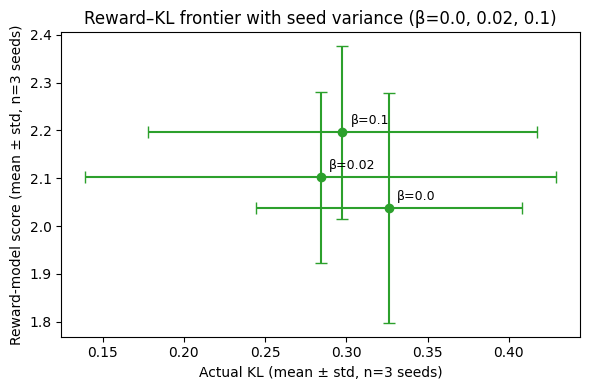
\includegraphics[width=\linewidth]{kl_seed_repeat_plot.png}
\caption{$\beta \in \{0, 0.02, 0.1\}$에 대한 reward--KL frontier(평균 $\pm$
표준편차, $n{=}3$ 시드). 오차 막대가 조건 간 평균 차이보다 크거나 비슷해,
이 규모에서는 $\beta$의 효과가 시드 분산과 뚜렷이 구분되지 않음을 보여준다.}
\label{fig:seedrepeat}
\end{figure}

표~\ref{tab:seedrepeat}와 그림~\ref{fig:seedrepeat}에서 $\beta$ 간 평균 reward 차이는 최대 $0.16$
($\beta{=}0.00$ 대 $\beta{=}0.10$)인 반면, 각 $\beta$ 내 시드 간 표준편차는
$0.18$--$0.24$로 그보다 크거나 비슷하다. 즉 이 실험 규모에서는 $\beta$를
바꿔서 얻는 평균적 차이가 같은 $\beta$를 다른 시드로 재현했을 때 생기는
차이보다 작다.

% =====================================================================
\section{Discussion}
\label{sec:discussion}
% =====================================================================

\subsection{PPO 미세조정이 baseline 보상을 넘지 못함}

표~\ref{tab:results}에서 보듯 6개 PPO 조건 모두 SFT baseline(2.545)보다
낮은 평균 보상(1.59--2.19)을 보였다. 이는 (i) 보상모델이 순위 데이터의
10\%만으로 학습되어 일반화 성능이 제한적이었을 가능성과, (ii) 10-episode
라는 극소 학습 예산이 안정적인 정책 개선에 애초에 불충분했을 가능성을
함께 시사한다. 이 결과는 $\beta$ 값과 무관하게 나타나므로, $\beta$ 자체의
효과라기보다 실험 규모의 한계로 해석하는 것이 합리적이다.

\subsection{반복 붕괴는 $\beta$가 아니라 SFT 단계에서 이어짐}

baseline(PPO 학습 전 SFT 모델) 자체가 이미 \texttt{max\_repetition=0.950}으로
심한 반복 경향을 보인다. PPO로 학습한 6개 조건의 \texttt{max\_repetition}도
$0.794$--$0.952$로 baseline과 비슷한 범위에 머물러 있어, 관측된 반복 붕괴가
PPO나 $\beta$가 새로 유발한 문제라기보다 KoGPT2(125M)를 소량의 데이터로
SFT한 데서 이미 존재하던 경향을 PPO가 그대로 물려받은 것으로 해석된다.
다만 6개 조건 중 $\beta{=}0.02$(0.794)와 $\beta{=}1.00$(0.800)이 상대적으로
가장 낮은 \texttt{max\_repetition}을 보여, $\beta$가 아주 작거나 아주 클 때
오히려 반복이 다소 완화되는 경향이 약하게 관측된다.

\subsection{$\beta$의 효과는 시드 분산 규모 내에 있음}

\S\ref{sec:seedrepeat}의 시드 반복 실험(표~\ref{tab:seedrepeat})은 이 해석을
뒷받침한다. 동일 시드 내에서 $\beta{=}0, 0.02, 0.1$을 바꿔도 reward, KL,
distinct-2가 거의 변하지 않는 반면(예: seed 2에서 $\beta{=}0.00$과
$\beta{=}0.02$의 reward는 소수점 자리까지 동일했다), 시드를 바꾸면 그보다
큰 차이가 발생했다. 이는 조건당 단일 시드로 얻은 reward--KL frontier가
대규모 연구에서 보고된 매끈한 곡선~\cite{ziegler2019finetuning,
stiennon2020learning}과 다르게 나타날 수 있음을 설명하며, KL 정규화의
이론적 효과가 신뢰성 있게 관측되려면 조건당 다중 시드와 더 큰 학습
예산이 필요함을 시사한다.

\subsection{Corpus 단위 distinct-n의 사각지대}

$\beta{=}0.05$는 distinct-2가 $0.764$로 baseline(0.762)과 사실상 같거나
오히려 높아, 식~\eqref{eq:selection}의 다양성 하한선($0.7\times 0.762 =
0.533$)을 여유 있게 통과한다. 그러나 \texttt{max\_repetition}은
baseline과 동일한 $0.950$으로, 30개 평가 응답 중 적어도 하나는 여전히
심하게 반복되는 퇴화 응답임을 의미한다. 즉 corpus 전체를 풀링한
distinct-2만 보면 이 조건은 "다양성이 충분하다"고 잘못 판정되지만,
샘플 단위 반복률(식~\eqref{eq:reprate})과 퇴화 판정(식~\eqref{eq:degenerate})을
함께 보면 실제로는 후보에서 제외되어야 함이 드러난다. 이는 Holtzman et
al.~\cite{holtzman2020curious}이 지적한 corpus 단위 다양성 지표의 한계를
본 실험에서 수치로 확인한 사례이며, Gao et al.~\cite{gao2023scaling}이
논의하는 것처럼 제한된 데이터로 학습된 보상모델·다양성 지표만으로 모델을
선택하는 것의 위험성을 뒷받침한다.

% =====================================================================
\section{Limitations}
% =====================================================================

본 연구는 다음과 같은 한계를 가진다: (i) 주 스윕(6개 조건)은 조건당 단일
시드로만 수행되었고, 시드 반복은 $\beta \in \{0, 0.02, 0.1\}$ 세 조건(추가
시드 2개, 총 3회 관측)에 대해서만 수행되었다, (ii) 학습 예산이 극히 작아
(10 episode) $\beta$의 장기적 효과를 완전히 관측하지 못했을 수 있다,
(iii) 보상모델이 순위 데이터의 10\%만으로 학습되어 보상 신호 자체의
신뢰도가 제한적일 수 있다, (iv) 125M 파라미터의 소형 모델(KoGPT2)을
사용하여 대규모 모델에서의 일반화 가능성은 별도 검증이 필요하다, (v)
평가 프롬프트가 30개로 제한적이다.

% =====================================================================
\section{Conclusion and Future Work}
% =====================================================================

본 연구는 KoChatGPT PPO 튜토리얼에서 검증되지 않았던 KL 계수 $\beta$를
6개 조건에 대해 스윕하고, 그중 3개 조건을 추가 시드로 반복하여 검증하였다.
그 결과 (i) 본 실험 규모에서는 PPO로 학습한 모든 조건이 SFT baseline보다
낮은 보상을 보였고, (ii) 샘플 단위 반복 붕괴는 $\beta$가 아니라 SFT
단계에서부터 이어지는 경향으로 보이며, (iii) 시드 반복 실험에서 $\beta$
간 차이가 시드 간 차이보다 작아 이 규모에서는 $\beta$의 효과가 시드
분산에 가려질 수 있음을, (iv) corpus 단위 distinct-n이 실제로 존재하는
샘플 단위 반복 붕괴를 놓치는 구체적 사례를 확인하였다. 향후 연구로는
(1) 6개 조건 전체에 대한 다중 시드 반복을 통한 통계적으로 유의한
reward--KL frontier 재현, (2) 보상모델 학습에 사용하는 순위 데이터
비율 확대, (3) Ziegler et al.~\cite{ziegler2019finetuning}이 제안한
adaptive KL controller의 적용, (4) 더 큰 모델과 학습 예산에서의 재현을
제안한다.

% =====================================================================
\bibliographystyle{IEEEtran}
\bibliography{references}

\end{document}
